\chapter{Association rules}


\section{Frequent itemset}

\begin{description}
    \item[Itemset] \marginnote{Itemset}
        Collection of one or more items (e.g. $\{ \text{milk}, \text{bread}, \text{diapers} \}$).

    \item[K-itemset] \marginnote{K-itemset}
        Itemset with $k$ items.

    \item[Support count] \marginnote{Support count}
        Number of occurrences of an itemset in a dataset.
        \begin{example}
            \phantom{}\\
            \begin{minipage}{0.4\textwidth}
                Given the following transactions:
                \begin{center}
                    \begin{tabular}{|c|l|}
                        \hline
                        1 & bread, milk \\
                        2 & beer, bread, diaper, eggs \\
                        3 & beer, coke, diaper, milk \\
                        \textbf{4} & \textbf{beer, bread, diaper, milk} \\
                        \textbf{5} & \textbf{bread, coke, diaper, milk} \\
                        \hline
                    \end{tabular}
                \end{center}
            \end{minipage}
            \begin{minipage}{0.5\textwidth}
                The support count of the itemset containing bread, diapers and milk is:
                \[ \sigma(\{ \text{bread}, \text{diapers}, \text{milk} \}) = 2 \]
            \end{minipage}
        \end{example}

        \item[Association rule] \marginnote{Association rule}
        Given two itemsets $A$ and $C$, an association rule has form:
        \[ A \rightarrow C \]
        It means that there are transactions in the dataset where $A$ and $C$ co-occur. 
        Note that it is not strictly a logical implication.

    \item[Metrics] \phantom{}
        \begin{description}
            \item[Support] \marginnote{Support}
            Given $N$ transactions, the support of an itemset $A$ is:
            \[ \texttt{sup}(A) = \frac{\sigma(A)}{N} \]
            The support of an association rule $A \rightarrow C$ is:
            \[ \texttt{sup}(A \rightarrow C) = \texttt{sup}(A \cup C) = \frac{\sigma(A \cup C)}{N} \]

            Low support implies random associations.

            \begin{description}
                \item[Frequent itemset] \marginnote{Frequent itemset}
                    Itemset whose support is at least a given threshold.
            \end{description}
    
        \item[Confidence] \marginnote{Confidence}
            Given an association rule $A \rightarrow C$, its confidence is given by:
            \[ \texttt{conf}(A \rightarrow C) = \frac{\sigma(A \cup C)}{\sigma(A)} \in [0, 1] \]

            Low confidence implies low reliability.

            \begin{theorem}
                The confidence of $A \rightarrow C$ can be computed given the supports of $A \rightarrow C$ and $A$:
                \[ \texttt{conf}(A \rightarrow C) = \frac{\texttt{sup}(A \rightarrow C)}{\texttt{sup}(A)} \]
            \end{theorem}
    \end{description}

    \item[Association rule mining] \marginnote{Association rule mining}
        Given $N$ transactions and two thresholds \texttt{min\_sup} and \texttt{min\_conf},
        association rule mining finds all the rules $A \rightarrow C$ such that:
        \[ \begin{split}
            \texttt{sup}(A \rightarrow C) &\geq \texttt{min\_sup} \\
            \texttt{conf}(A \rightarrow C) &\geq \texttt{min\_conf}
        \end{split} \]

        This can be done in two steps:
        \begin{enumerate}
            \item \marginnote{Frequent itemset generation}
                Determine the itemsets with $\text{support} \geq \texttt{min\_sup}$ (frequent itemsets).
            \item \marginnote{Rule generation}
                Determine the association rules with $\text{confidence} \geq \texttt{min\_conf}$.
        \end{enumerate}
\end{description}



\section{Frequent itemset generation}

\subsection{Brute force}
Given $D$ items, there are $2^D$ possible itemsets.
To compute the support of a single itemset, the complexity is $O(NW)$ where 
$N$ is the number of transactions and $W$ is the width of the largest transaction.
Listing all the itemsets and computing their support have an exponential complexity of $O(NW2^D)$.


\subsection{Apriori principle}

\begin{theorem} \marginnote{Apriori principle}
    If an itemset is frequent, then all of its subsets are frequent.

    \begin{proof}
        By the definition of support, it holds that:
        \[ \forall X, Y: (X \subseteq Y) \Rightarrow (\texttt{sup}(X) \geq \texttt{sup}(Y)) \]

        In other words, the support metric is anti-monotone.
    \end{proof}
\end{theorem}

\begin{corollary}
    If an itemset is infrequent, then all of its supersets are infrequent.
\end{corollary}

\begin{example} \phantom{}
    \begin{center}
        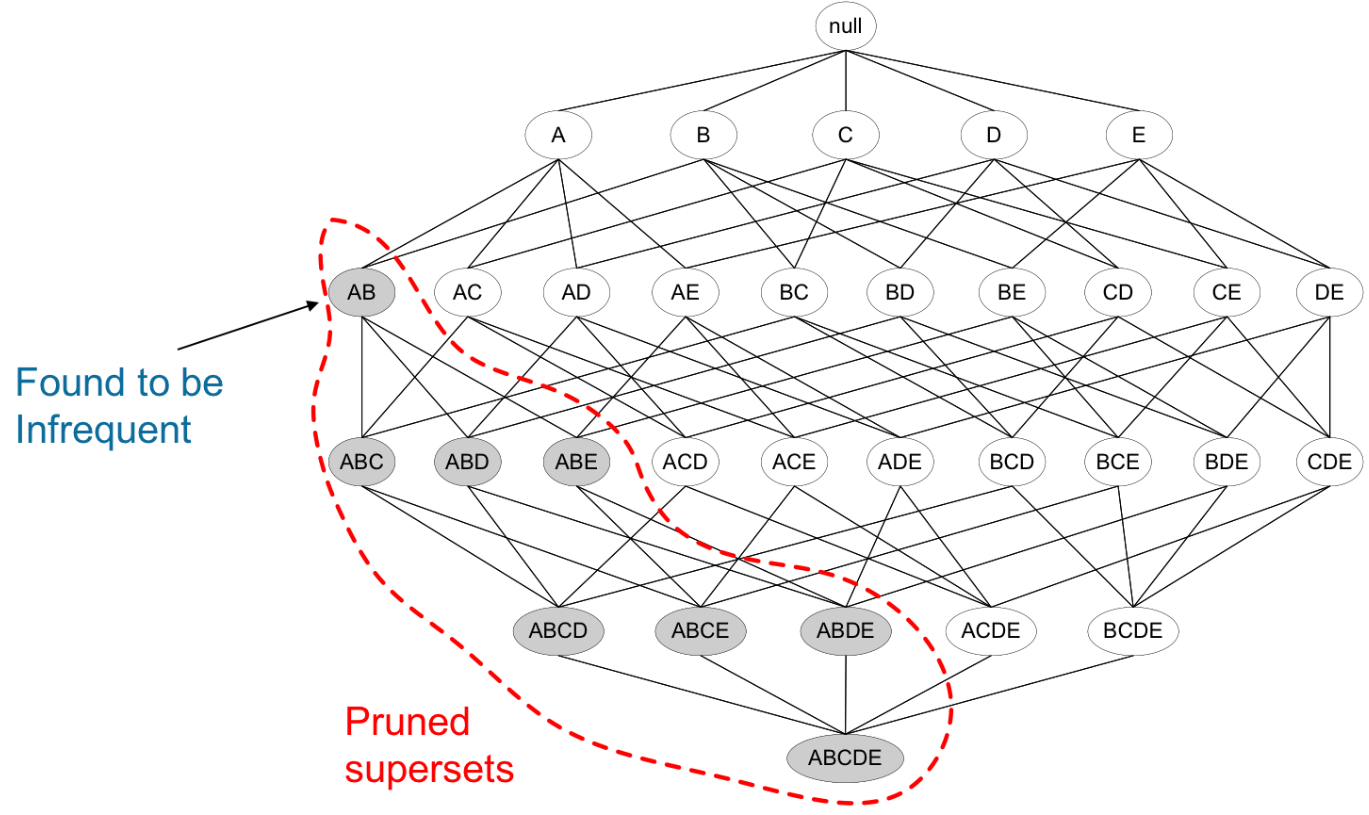
\includegraphics[width=0.6\textwidth]{img/itemset_apriori.png}
    \end{center}
\end{example}

\begin{algorithm}[H]
\caption{Apriori principle}
\begin{lstlisting}[mathescape=true]
def candidatesGeneration(freq_itemsets$_k$):
    candidate_itemsets$_{k+1}$ = selfJoin(freq_itemsets$_k$)
    for itemset in candidate_itemsets$_{k+1}$:
        for sub in subsetsOfSize($k$, itemset):
            if sub not in freq_itemsets$_k$:
                candidate_itemsets$_{k+1}$.remove(itemset)
    return candidate_itemsets$_{k+1}$

def aprioriItemsetGeneration(transactions, min_sup):
    freq_itemsets$_1$ = itemsetsOfSize(1, transactions)
    k = 1
    while freq_itemsets$_1$ is not null:
        candidate_itemsets$_{k+1}$ = candidatesGeneration(freq_itemsets$_k$)
        freq_itemsets$_{k+1}$ = $\{ c \in \texttt{candidate\_itemsets}_{k+1} \mid \texttt{sup(}c\texttt{)} \geq \texttt{min\_sup} \}$
        k += 1
    return freq_itemsets$_k$
\end{lstlisting}
\end{algorithm}

\begin{description}
    \item[Complexity]
        The complexity of the apriori principle depends on:
        \begin{itemize}
            \item The choice of the support threshold.
            \item The number of unique items.
            \item The number and the width of the transactions.
        \end{itemize}
\end{description}



\section{Rule generation}

\subsection{Brute force}
Given a frequent $k$-itemset $L$, there are $2^k-2$ possible association rules ($-2$ as $L \rightarrow \varnothing$ and $\varnothing \rightarrow L$ can be ignored).
For each possible rule, it is necessary to compute the confidence. The overall complexity is exponential.

\subsection{Apriori principle}

\begin{theorem} \marginnote{Apriori principle}
    Without loss of generality, consider an itemset $\{ A, B, C, D \}$.
    It holds that:
    \[ \texttt{conf}(ABC \rightarrow D) \geq \texttt{conf}(AB \rightarrow CD) \geq \texttt{conf}(A \rightarrow BCD) \]
\end{theorem}

\begin{example} \phantom{}
    \begin{center}
        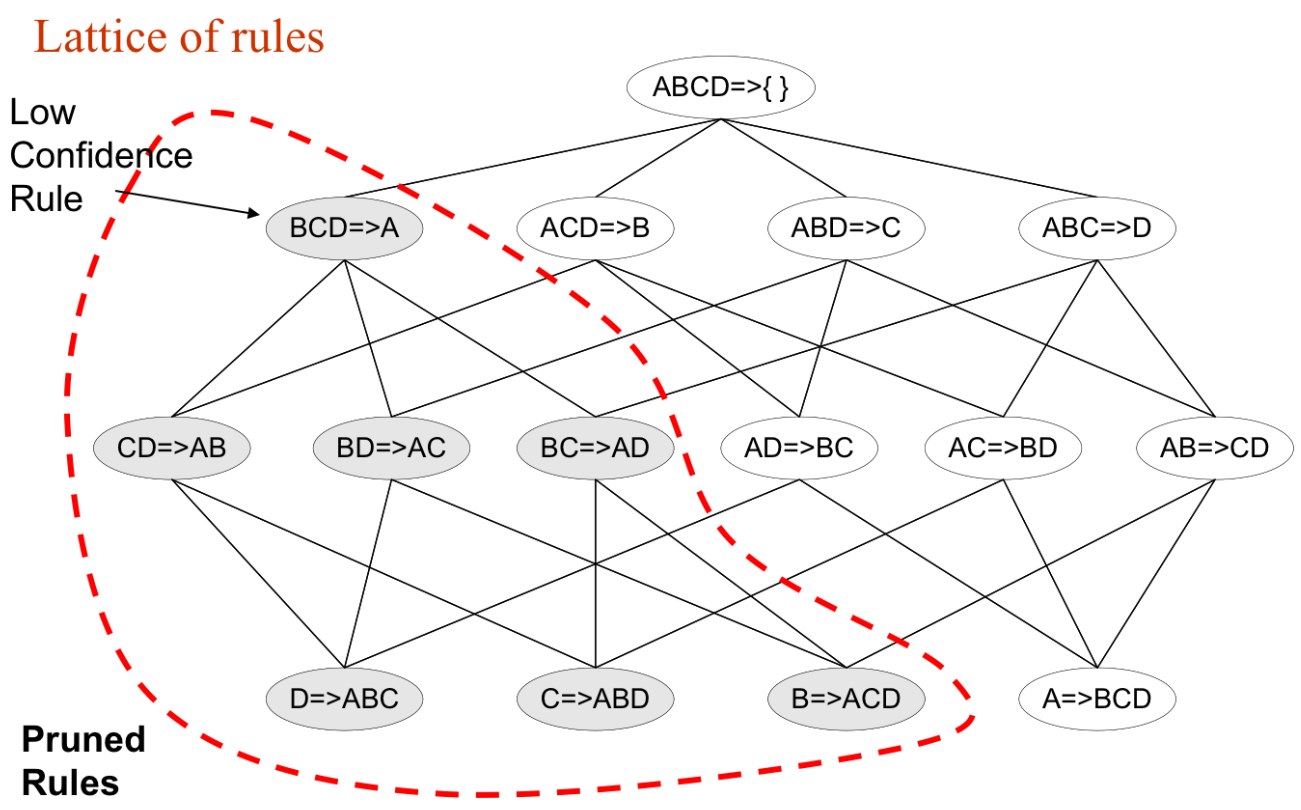
\includegraphics[width=0.5\textwidth]{img/rules_apriori.png}
    \end{center}
\end{example}



\section{Interestingness measures}

\begin{description}
    \item[Contingency table] \marginnote{Contingency table}
        Given an association rule $A \rightarrow C$, its contingency table is defined as:
        \begin{center}
            \def\arraystretch{1.1}
            \begin{tabular}{c|c|c|c}
                & $C$ & $\overline{C}$ & \\
                \hline
                $A$ & $\prob{A \land C}$ & $\prob{A \land \overline{C}}$ & $\prob{A}$ \\
                \hline
                $\overline{A}$ & $\prob{\overline{A} \land C}$ & $\prob{\overline{A} \land \overline{C}}$ & $\prob{\overline{A}}$ \\
                \hline
                & $\prob{C}$ & $\prob{\overline{C}}$ & 100 \\
            \end{tabular}
        \end{center}
\end{description}

\begin{remark}
    Confidence can be misleading.
    \begin{example} \phantom{}\\
        \begin{minipage}[t]{0.36\textwidth}
            Given the following contingency table:
            \begin{center}
                \begin{tabular}{c|c|c|c}
                                                & coffee    & $\overline{\text{coffee}}$ & \\
                    \hline
                    tea                         & 15        & 5                     & 20 \\
                    \hline
                    $\overline{\text{tea}}$     & 75        & 5                     & 80 \\
                    \hline
                                                & 90        & 10                    & 100 \\
                \end{tabular}
            \end{center}
        \end{minipage}
        \hspace{0.5cm}
        \begin{minipage}[t]{0.6\textwidth}
            We have that:
            \[ \texttt{conf}(\text{tea} \rightarrow \text{coffee}) = \frac{\texttt{sup}(\text{tea}, \text{coffee})}{\texttt{sup}(\text{tea})} = \frac{15}{20} = 0.75 \]
            But, we also have that:
            \[ \prob{\text{coffee}} = 0.9 \hspace*{1cm} \prob{\text{coffee} \mid \overline{\text{tea}}} = \frac{75}{80} = 0.9375 \]
            So, despite the high confidence of $(\text{tea} \rightarrow \text{coffee})$,
            the probability of coffee increases in absence of tea.
        \end{minipage}
    \end{example}
\end{remark}


\subsection{Statistical-based measures}

Measures that take into account the statistical independence of the items.

\begin{description}
    \item[Lift] \marginnote{Lift}
        \[ \texttt{lift}(A \rightarrow C) = \frac{\texttt{conf}(A \rightarrow C)}{\texttt{sup}(C)} = \frac{\prob{A \land C}}{\prob{A}\prob{C}} \]

        If $\texttt{lift}(A \rightarrow C) = 1$, then $A$ and $C$ are independent.
    
    \item[Leverage] \marginnote{Leverage}
        \[ \texttt{leve}(A \rightarrow C) = \texttt{sup}(A \cup C) - \texttt{sup}(A)\texttt{sup}(C) = \prob{A \land C} - \prob{A}\prob{C} \]
        
        If $\texttt{leve}(A \rightarrow C) = 0$, then $A$ and $C$ are independent.
    
    \item[Conviction] \marginnote{Conviction}
        \[ \texttt{conv}(A \rightarrow C) = \frac{1 - \texttt{sup}(C)}{1 - \texttt{conf}(A \rightarrow C)} = \frac{\prob{A}(1-\prob{C})}{\prob{A}-\prob{A \land C}} \]
\end{description}

\begin{table}[H]
    \centering
    \begin{tabular}{c|p{10cm}}
        \hline
        \textbf{Metric} & \textbf{Interpretation} \\
        \hline
        High support        & The rule applies to many transactions. \\
        \hline
        High confidence     & The chance that the rule is true for some transactions is high. \\
        \hline
        High lift           & Low chance that the rule is just a coincidence. \\
        \hline
        High conviction     & The rule is violated less often compared to the case when the antecedent and consequent are independent. \\
        \hline
    \end{tabular}
    \caption{Intuitive interpretation of the measures}
\end{table}



\section{Multi-dimensional association rules}

\begin{description}
    \item[Mono-dimensional events] \marginnote{Mono-dimensional events}
        Represented as transactions. Each event contains items that appear together.
        
    \item[Multi-dimensional events] \marginnote{Multi-dimensional events}
        Represented as tuples. Each event contains the values of its attributes.

    \item[Mono/Multi-dimensional equivalence] \marginnote{Equivalence}
        Mono-dimensional events can be converted into multi-dimensional events and vice versa.

        To transform quantitative attributes, it is usually useful to discretize them.

        \begin{example}[Multi to mono] \phantom{}\\
            \begin{minipage}{0.35\textwidth}
                \begin{center}
                    \begin{tabular}{c|c|c}
                        \textbf{Id} & \textbf{co2} & \textbf{tin\_oxide} \\
                        \hline
                        1 & high & medium \\
                        2 & medium & low \\
                    \end{tabular}
                \end{center}
            \end{minipage}
            $\rightarrow$
            \begin{minipage}{0.48\textwidth}
                \begin{center}
                    \begin{tabular}{c|c}
                        \textbf{Id} & \textbf{Transaction} \\
                        \hline
                        1 & $\{ \text{co2/high}, \text{tin\_oxide/medium} \}$ \\
                        2 & $\{ \text{co2/medium}, \text{tin\_oxide/low} \}$ \\
                    \end{tabular}
                \end{center}
            \end{minipage}
        \end{example}

        \begin{example}[Mono to multi] \phantom{}\\
            \begin{minipage}{0.35\textwidth}
                \begin{center}
                    \begin{tabular}{c|c|c|c|c}
                        \textbf{Id} & \textbf{a} & \textbf{b} & \textbf{c} & \textbf{d} \\
                        \hline
                        1 & yes & yes & no & no \\
                        2 & yes & no & yes & no \\
                    \end{tabular}
                \end{center}
            \end{minipage}
            $\leftarrow$
            \begin{minipage}{0.30\textwidth}
                \begin{center}
                    \begin{tabular}{c|c}
                        \textbf{Id} & \textbf{Transaction} \\
                        \hline
                        1 & $\{ \text{a}, \text{b} \}$ \\
                        2 & $\{ \text{a}, \text{c} \}$ \\
                    \end{tabular}
                \end{center}
            \end{minipage}
        \end{example}

\end{description}



\section{Multi-level association rules}
Organize items into a hierarchy.

\begin{description}
    \item[Specialized to general] \marginnote{Specialized to general} 
        Generally, the support of the rule increases.
        \begin{example}
            From $(\text{apple} \rightarrow \text{milk})$ to $(\text{fruit} \rightarrow \text{dairy})$
        \end{example}

    \item[General to specialized] \marginnote{General to specialized} 
        Generally, the support of the rule decreases.
        \begin{example}
            From $(\text{fruit} \rightarrow \text{dairy})$ to $(\text{apple} \rightarrow \text{milk})$
        \end{example}

    \item[Redundant level] \marginnote{Redundant level}
        A more specialized rule in the hierarchy is redundant if its confidence is similar to the one of a more general rule.

    \item[Multi-level association rule mining] \marginnote{Multi-level association rule mining}
        Run association rule mining on different levels of abstraction (general to specialized).
        At each level, the support threshold is decreased.
\end{description}